\section{XMWidget\-List  Class Reference}
\label{classXMWidgetList}\index{XMWidgetList@{XMWidget\-List}}
{\tt \#include $<$XMWlist.h$>$}

Inheritance diagram for XMWidget\-List::\begin{figure}[H]
\begin{center}
\leavevmode
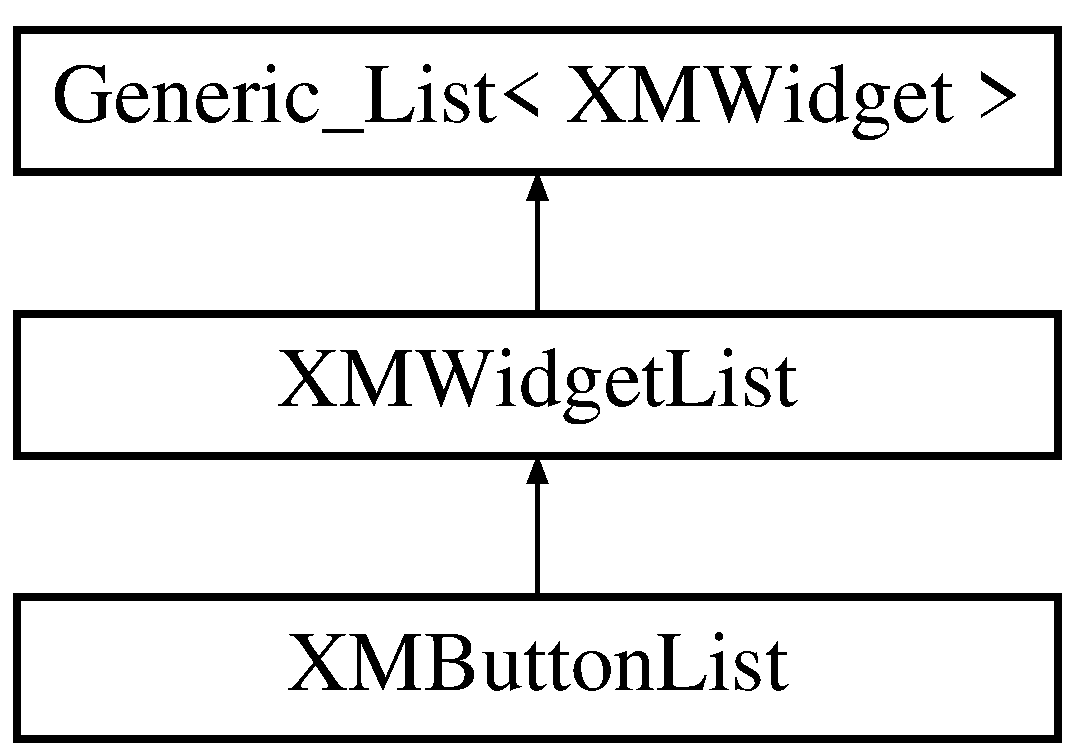
\includegraphics[height=3cm]{classXMWidgetList}
\end{center}
\end{figure}
\subsection*{Public Methods}
\begin{CompactItemize}
\item 
{\bf XMWidget\-List} (int num=LIST\_\-DEFAULT\_\-SIZE)
\item 
void {\bf Set\-Attribute} (String attribute, Xt\-Arg\-Val value)
\item 
void {\bf Set\-Attribute} (String attribute, void $\ast$value)
\end{CompactItemize}


\subsection{Constructor \& Destructor Documentation}
\index{XMWidgetList@{XMWidget\-List}!XMWidgetList@{XMWidgetList}}
\index{XMWidgetList@{XMWidgetList}!XMWidgetList@{XMWidget\-List}}
\subsubsection{\setlength{\rightskip}{0pt plus 5cm}XMWidget\-List::XMWidget\-List (int {\em num} = LIST\_\-DEFAULT\_\-SIZE)\hspace{0.3cm}{\tt  [inline]}}\label{classXMWidgetList_a0}




Definition at line 374 of file XMWlist.h.

References LIST\_\-DEFAULT\_\-SIZE.

\subsection{Member Function Documentation}
\index{XMWidgetList@{XMWidget\-List}!SetAttribute@{SetAttribute}}
\index{SetAttribute@{SetAttribute}!XMWidgetList@{XMWidget\-List}}
\subsubsection{\setlength{\rightskip}{0pt plus 5cm}void XMWidget\-List::Set\-Attribute (String {\em attribute}, void $\ast$ {\em value})}\label{classXMWidgetList_a2}




Definition at line 322 of file XMWlist.cpp.

References Generic\_\-List$<$ XMWidget $>$::Exists(), Generic\_\-List$<$ XMWidget $>$::Init\-Iteration(), Generic\_\-List$<$ XMWidget $>$::Next(), and XMWidget::Set\-Attribute().\index{XMWidgetList@{XMWidget\-List}!SetAttribute@{SetAttribute}}
\index{SetAttribute@{SetAttribute}!XMWidgetList@{XMWidget\-List}}
\subsubsection{\setlength{\rightskip}{0pt plus 5cm}void XMWidget\-List::Set\-Attribute (String {\em attribute}, Xt\-Arg\-Val {\em value})}\label{classXMWidgetList_a1}




Definition at line 312 of file XMWlist.cpp.

References Generic\_\-List$<$ XMWidget $>$::Exists(), Generic\_\-List$<$ XMWidget $>$::Init\-Iteration(), Generic\_\-List$<$ XMWidget $>$::Next(), and XMWidget::Set\-Attribute().

Referenced by XMButton\-List::Disable(), and XMButton\-List::Enable().

The documentation for this class was generated from the following files:\begin{CompactItemize}
\item 
{\bf XMWlist.h}\item 
{\bf XMWlist.cpp}\end{CompactItemize}
